\documentclass[border=10pt]{standalone}
\usepackage{tikz}
\usepackage[svgnames]{xcolor}
\usepackage{amsmath,amsfonts,amssymb}
\usetikzlibrary{positioning, calc, fit, arrows.meta, backgrounds, shapes.geometric}

\begin{document}
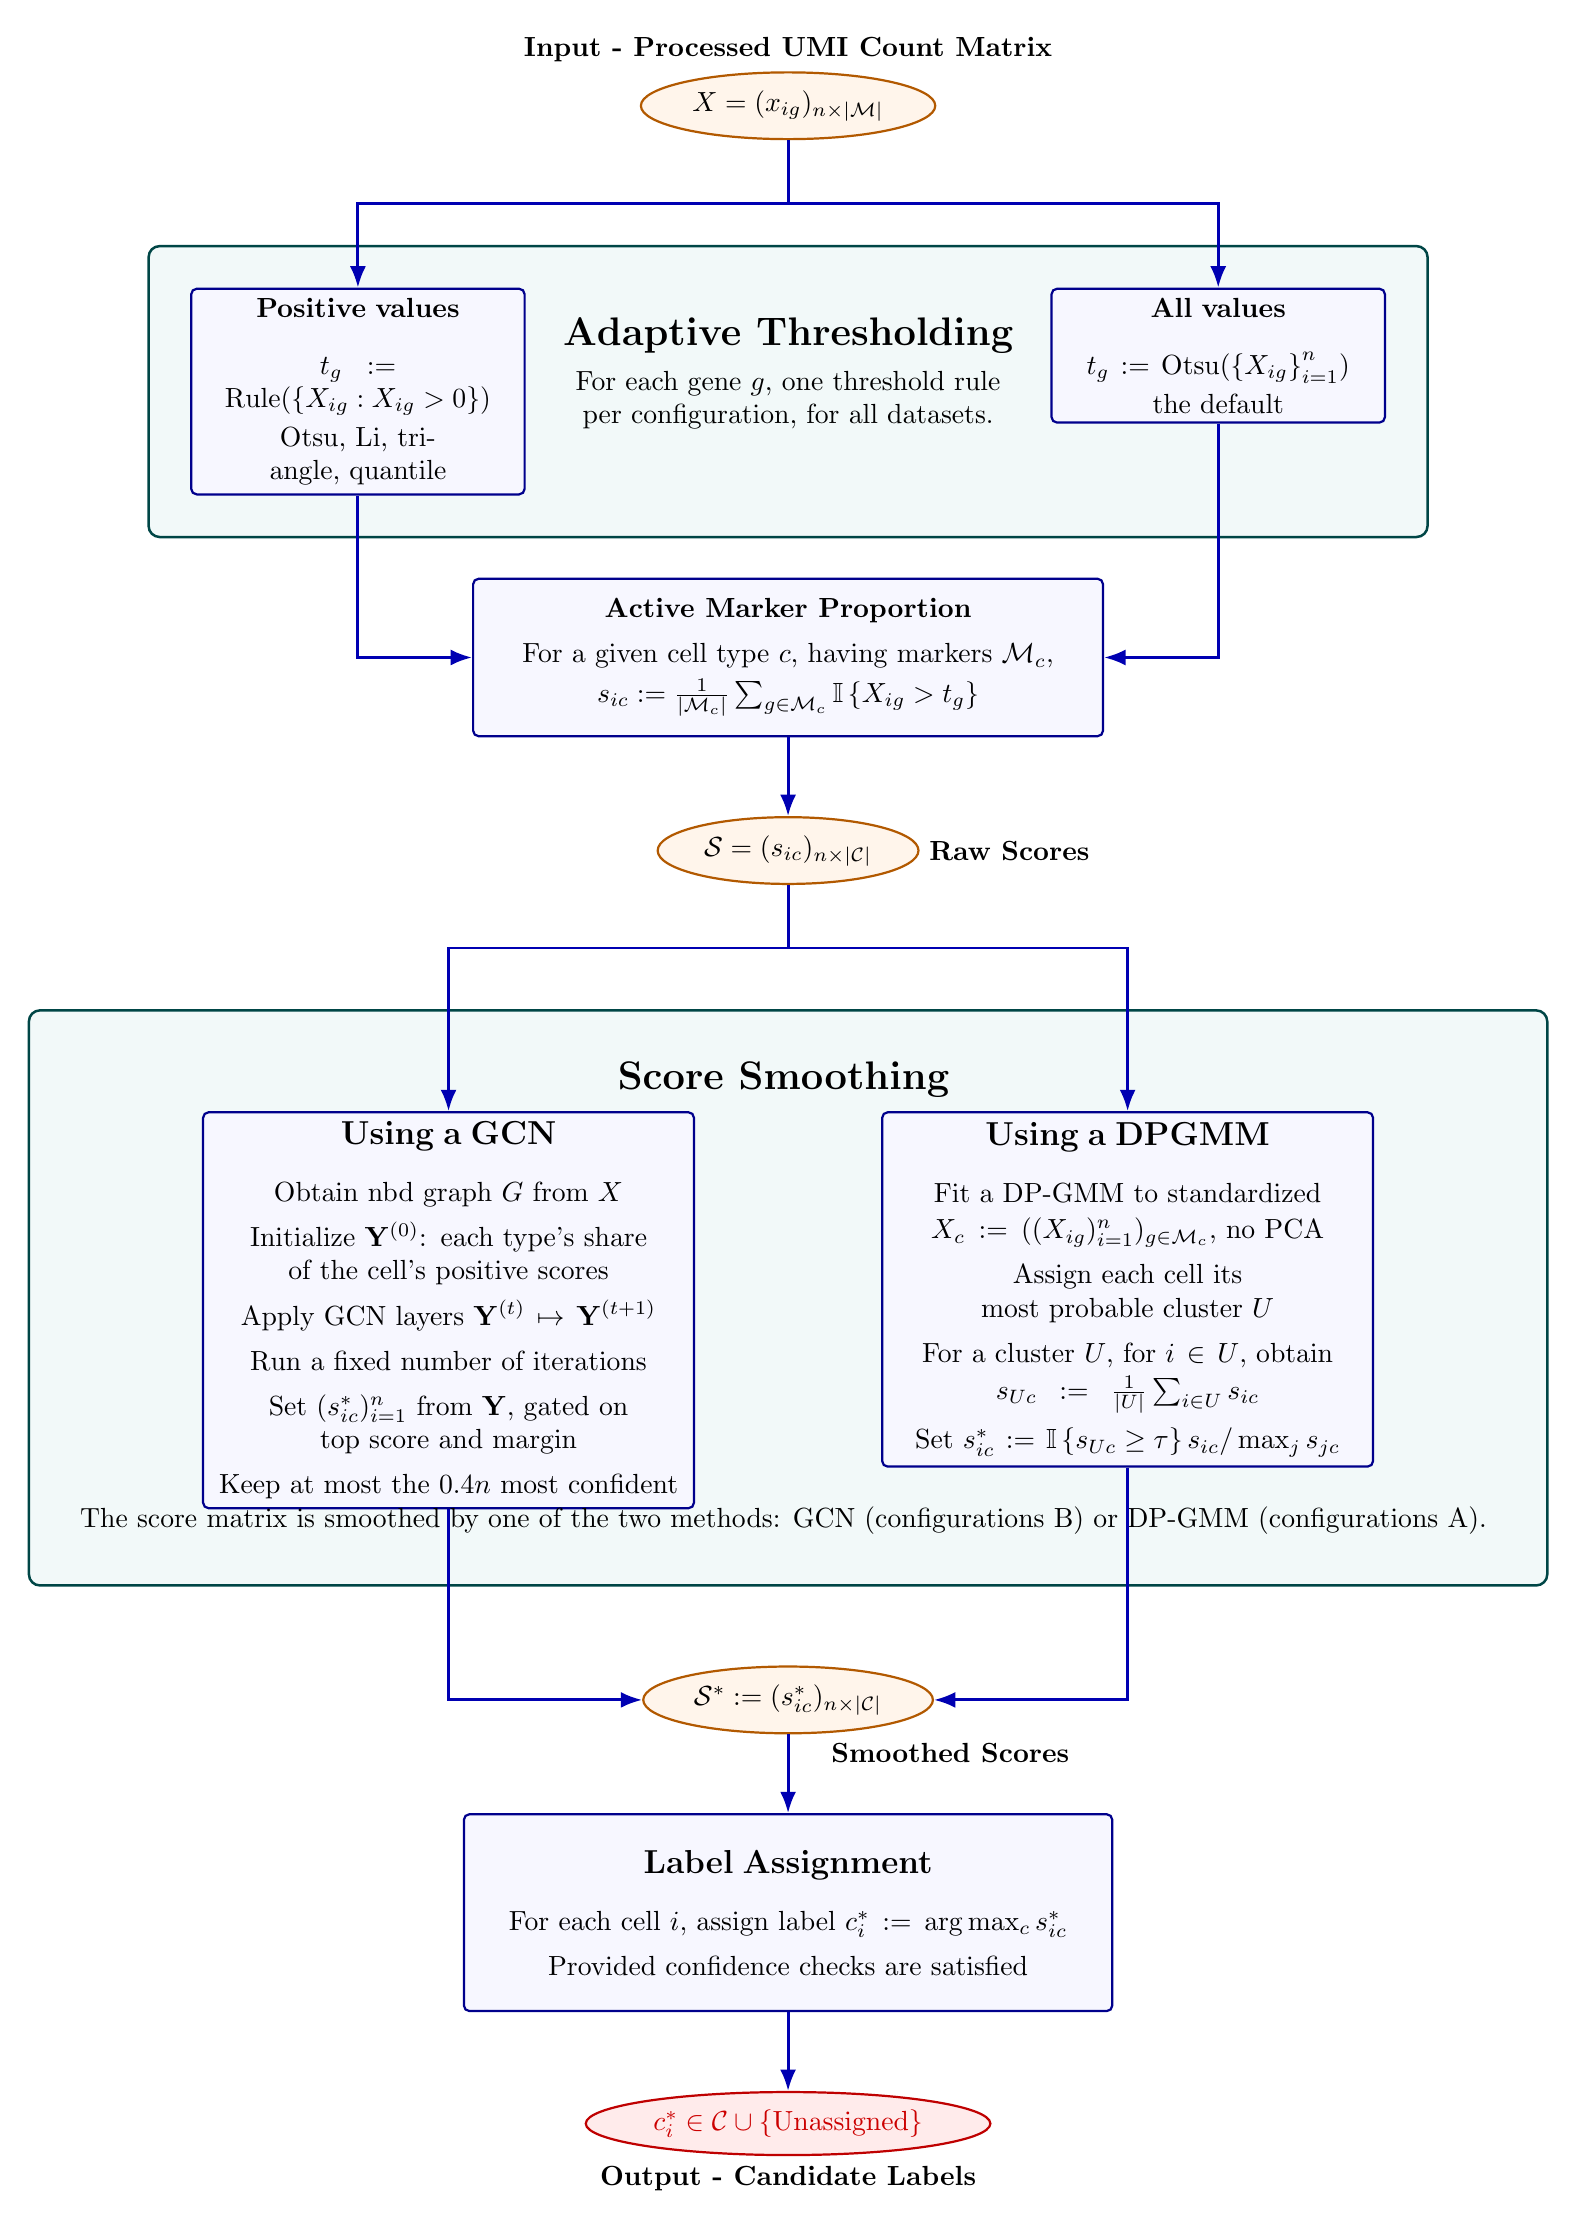
\begin{tikzpicture}[
    >=Latex,
    box/.style={draw=blue!55!black, line width=0.8pt, rectangle, align=center, minimum height=1.2cm, minimum width=2.5cm, fill=blue!3, rounded corners=2pt},
    container/.style={draw=teal!55!black, line width=0.9pt, rectangle, inner sep=15pt, align=center, rounded corners=4pt, fill=teal!5},
    var/.style={draw=orange!70!black, line width=0.8pt, ellipse, align=center, inner sep=3pt, fill=orange!8},
    flow/.style={->, line width=1.05pt, draw=blue!70!black},
    bypass/.style={->, dashed, line width=1.0pt, draw=red!70!black},
    txt/.style={align=center, font=\Large\bfseries}
  ]

  
  \node[var, label=above:\textbf{Input - Processed UMI Count Matrix}] (input) {$X = (x_{ig})_{n \times |\mathcal{M}|}$};

  
  
  \node[box, below left=2cm and 2cm of input, text width=4cm, minimum height=1.5cm] (quantile) {\textbf{Positive values}\\[2ex] $t_g := \mathrm{Rule}(\left\{X_{ig} : X_{ig} > 0\right\})$\\[0.5ex] Otsu, Li, triangle, quantile};
  \node[box, below right=2cm and 2cm of input, text width=4cm, minimum height=1.5cm] (otsu) {\textbf{All values}\\[2ex] $t_g := \mathrm{Otsu}(\left\{X_{ig}\right\}_{i=1}^n)$\\[0.5ex] the default};

  
  \node[align=center] (adapt_label) at ($(quantile)!0.5!(otsu)$) {
    {\Large\bfseries Adaptive Thresholding} \\[1ex] For each gene $g$, one threshold rule\\ per configuration, for all datasets.
  };

  
  \begin{scope}[on background layer]
    \node[container, fit=(quantile) (otsu) (adapt_label), align=center] (adapt_thresh) {};
  \end{scope}

  
  \node[box, below=0.5cm of adapt_thresh, minimum height=2cm, minimum width=8cm] (sic) {
    {\bfseries Active Marker Proportion}\\[1ex]
    For a given cell type $c$, having markers $\mathcal{M}_c$,\\[0.5ex]
    $s_{ic} := \frac{1}{|\mathcal{M}_c|}\sum_{g \in \mathcal{M}_c} \mathbb{I}\left\{X_{ig} > t_g\right\}$
  };

  
  \node[var, below=1cm of sic, label=right:\textbf{Raw Scores}] (raw_scores) {$\mathcal{S} = (s_{ic})_{n \times |\mathcal{C}|}$};

  
  \node[box, below left=3cm and 0cm of raw_scores, text width=6cm, minimum height=4.5cm] (gcn) {
    {\large\bfseries Using a GCN}\\[2ex]
    Obtain nbd graph $G$ from $X$\\[1ex]
    Initialize $\mathbf{Y}^{(0)}$: each type's share\\ of the cell's positive scores\\[1ex]
    Apply GCN layers $\mathbf{Y}^{(t)} \mapsto \mathbf{Y}^{(t+1)}$\\[1ex]
    Run a fixed number of iterations \\[1ex]
    Set $(s_{ic}^*)_{i=1}^n$ from $\mathbf{Y}$, gated on\\ top score and margin\\[1ex]
    Keep at most the $0.4n$ most confident
  };
  \node[box, below right=3cm and 0cm of raw_scores, text width=6cm, minimum height=4.5cm] (dpgmm) {
    {\large\bfseries Using a DPGMM}\\[2ex]
    Fit a DP-GMM to standardized \\[0.3ex] $X_c := ((X_{ig})_{i=1}^n)_{g \in \mathcal{M}_c}$, no PCA \\[1ex]
    Assign each cell its most probable cluster $U$ \\[1ex]
    For a cluster $U$, for $i \in U$, obtain \\[0.3ex] $s_{Uc} := \frac{1}{|U|}\sum_{i \in U} s_{ic}$ \\[1ex]
    Set $s_{ic}^* := \mathbb{I}\left\{s_{Uc} \geq \tau\right\} s_{ic} / \max_j s_{jc}$
  };

  
  \node[align=center] (smooth_header) at ([yshift=2.8cm]$(gcn)!0.5!(dpgmm)$) {
    {\Large\bfseries Score Smoothing}
  };
  \node[align=center] (smooth_desc) at ([yshift=-2.8cm]$(gcn)!0.5!(dpgmm)$) {
    The score matrix is smoothed by one of the two methods: GCN (configurations B) or DP-GMM (configurations A).
  };

  
  \begin{scope}[on background layer]
    \node[container, fit=(gcn) (dpgmm) (smooth_header) (smooth_desc)] (smoothing) {};
  \end{scope}

  
  \node[var, below=1cm of smoothing, label=below right:\textbf{Smoothed Scores}] (smoothed_scores) {$\mathcal{S}^* := (s_{ic}^*)_{n \times |\mathcal{C}|}$};

  
  \node[box, below=1cm of smoothed_scores, text width=8cm, minimum height=2.5cm] (labelling) {
    {\large\bfseries Label Assignment}\\[2ex]
    For each cell $i$, assign label $c_i^* := \arg\max_{c} s_{ic}^*$\\[1ex]
    Provided confidence checks are satisfied
  };

  
  \node[var, below=1cm of labelling, text=red!80!black, fill=red!8, draw=red!75!black, label=below:\textbf{Output - Candidate Labels}] (output) {$c_i^* \in \mathcal{C} \cup \{\text{Unassigned}\}$};

  
  \draw[flow] (input.south) -- ++(0,-0.8) -| (quantile.north);
  \draw[flow] (input.south) -- ++(0,-0.8) -| (otsu.north);

  \draw[flow] (quantile.south) |- (sic.west);
  \draw[flow] (otsu.south) |- (sic.east);

  \draw[flow] (sic.south) -- (raw_scores.north);

  \draw[flow] (raw_scores.south) -- ++(0,-0.8) -| (gcn.north);
  \draw[flow] (raw_scores.south) -- ++(0,-0.8) -| (dpgmm.north);

  \draw[flow] (gcn.south) |- (smoothed_scores.west);
  \draw[flow] (dpgmm.south) |- (smoothed_scores.east);

  \draw[flow] (smoothed_scores.south) -- (labelling.north);
  \draw[flow] (labelling.south) -- (output.north);

\end{tikzpicture}
\end{document}
